
\documentclass[12pt,a4paper]{report}

% ---------- Encoding & Language ----------
\usepackage[utf8]{inputenc}
\usepackage[T1]{fontenc}
\usepackage[english]{babel}
\usepackage[english]{datetime2}

% ---------- Page Geometry & Spacing ----------
\usepackage{geometry}
\geometry{margin=1in}
\usepackage{setspace}
\onehalfspacing

% ---------- Figures, Tables, Math ----------
\usepackage{graphicx}
\usepackage{booktabs}
\usepackage{tabularx}
\usepackage{float}
\usepackage{amsmath, amssymb}
\usepackage{array}
\usepackage{enumitem}
\usepackage{ragged2e}
\usepackage{algorithm}
\usepackage{algpseudocode} % If using algorithmic pseudocode syntax

\setlist[itemize]{nosep,leftmargin=*}    % compact lists inside cells
\newcolumntype{R}[1]{>{\RaggedLeft\arraybackslash}p{#1}} % right + top aligned column
\setlength{\arrayrulewidth}{0.4pt}       % border thickness (adjust if needed)
\renewcommand{\arraystretch}{1.05}       % row height (optional)

% ---------- Lists & Formatting ----------
\setlist{leftmargin=2em}
\usepackage{hyperref}
\hypersetup{
    colorlinks=true,
    linkcolor=blue,
    citecolor=blue,
    urlcolor=blue,
    pdfauthor={AIP491 G10},
    pdftitle={Adaptive Transfer Learning for Cold-Start Electric Vehicle Charging Demand Forecasting},
}

% ---------- Typography & Hyphenation ----------
\usepackage[protrusion=true,expansion=false]{microtype}
\setlength{\emergencystretch}{1.5em}

% ---------- frame of title page ----------
\usepackage{tikz}
\usetikzlibrary{arrows.meta,positioning}
\tikzset{every node/.append style={execute at begin node={\hyphenpenalty=10000\exhyphenpenalty=10000}}}
\newcommand{\pageframe}{%
  \begin{tikzpicture}[remember picture,overlay]
    \draw[line width=0.8pt]
      ([xshift=1cm,yshift=-1cm]current page.north west)
      rectangle
      ([xshift=-1cm,yshift=1cm]current page.south east);
  \end{tikzpicture}%
  \begin{tikzpicture}[remember picture,overlay]
    \draw[line width=0.8pt]
      ([xshift=1.1cm,yshift=-1.1cm]current page.north west)
      rectangle
      ([xshift=-1.1cm,yshift=1.1cm]current page.south east);
  \end{tikzpicture}%
}

\begin{document}

\hypersetup{pageanchor=false}
\begin{titlepage}
    \pageframe 
    \begin{center}
        \vspace*{-1cm} 
        
        % FPTU Logo
        
\includegraphics[width=0.6\linewidth]{Images/FPT University logo.png}

        \vspace*{0.25cm}
        
        % Adjusted title size to fit in one page
        \Large
        \textbf{Adaptive Transfer Learning for Cold-Start Electric Vehicle Charging Demand Forecasting}
 
        \vspace{0.2cm}
        \vfill
        \begin{table}[H]
        \large
        \centering
        \begin{tabular}{rl}
        Project group: & AIP491 G10 \\
        Team members: & Nguyen Manh Quyen \\
                      & Luong Duc Hung \\
                      & Tran Manh Hung \\
                      & Nguyen Huu Duc \\[0.6em]
        Supervisor:      & MSc. Do Thai Giang      
        \end{tabular}
        \end{table}
        \Large

        \vspace{0.25cm}
        \vfill
        \Large
        Bachelor of Artificial Intelligence\\
        % =========== DO NOT MODIFY, it automatic place the current date ==========
        FPT University - \DTMenglishmonthname{\month} \the\year\\
        % =========================================================================
    \end{center}
\end{titlepage}

\hypersetup{pageanchor=true}
%\input{Preamble/acknowledgement}
\chapter*{Abstract}
A charging location with only a few days of recorded demand offers little evidence about its daily pattern. This study asks how much a forecaster benefits from training at established locations and whether recent forecast errors indicate when to relax the influence of the source model. Using UrbanEV and CHARGED, we simulate cold start by limiting the initial target history to 7, 14 or 28 days. A gated recurrent unit uses the preceding 24 hours and known calendar features to predict hourly charging energy for the next day. We compare source initialization with target-only training, calibrating the initial training budget separately for each. We then compare fixed retention with online selection of the strength of a penalty on changes in the encoder representation. A separate experiment combines forecasts from two transferred models and tests the value of adapting their weights after observations arrive. On twelve additional UrbanEV targets, source initialization reduced mean absolute error by 29.80--33.35\% across the three history budgets. Across 21 historical combinations of dataset, city and history duration, confidence-guided retention selection yielded lower error than fixed retention in nine and lower error than selection by recent mean absolute error in eleven. Both the calibrated static mixture and the adaptive mixture improved on a single fixed-retention model in eighteen combinations. Adaptive fusion improved on the calibrated static blend in twelve. In a separate fourteen-day comparison on twelve UrbanEV targets, an equal-weight mixture came within 0.000007 kWh of the adaptive MAE. On 46 additional Development identifiers selected before evaluation at the 14-day budget, the estimated reductions in error from adaptive fusion were 0.67\% against single fixed retention and 0.36\% against static fusion when each dataset--city group received equal weight. Both uncertainty intervals included zero. The results support source initialization for the tested short histories. The benefit of adapting retention or forecast weights varied with the target group and the comparison method.

\vspace{0.5cm}
\noindent\textbf{Keywords:} electric vehicle charging, demand forecasting, transfer learning, cold start, online adaptation


\tableofcontents
\listoffigures
\listoftables
\clearpage

\chapter{Introduction}\label{chap:introduction}

\section{Background and Motivation}

Suppose a charging station has recorded one week of hourly energy use. At midnight it needs a demand forecast for each hour of the coming day. Its records contain at most one example of each weekday. If charging peaked at noon last Tuesday, the forecaster has little local evidence to tell whether that peak will recur. Records from established locations offer a way to learn daily patterns before fitting a model to the station.

In transfer learning, the established locations supply the source data and the station receiving the forecast is the target. Source training gives the target model a starting point. A separate decision arises as local measurements arrive: how closely should the model continue to follow the representation learned at the source? A short run of forecast errors might reveal a persistent difference between locations, or it might reflect a few unusual charging days. The distinction matters because changing the model in response affects forecasts issued before the next day's demand is known.

\section{Literature Review}

Narayana Gowda et al.\ compared transfer learning, model-agnostic meta-learning and conventional LSTM training for aggregate EV charging load with 10 or 20 days of target data~\cite{gowda2026}. Their results support using observations from other settings when the local record is short. Ali et al.\ examined transfer at the charging-site level with a temporal convolutional network that predicts several load quantiles~\cite{ali2024}. With two weeks of local data at the NREL site, they reported prediction interval coverage of 96.88\%. Coverage measures how often observations fall inside a forecast interval. The decision studied here requires a different quantity: the difference in hourly forecast error between two retention settings on the same dates.

Recent work also considers how a station's demand changes over time. Chenghan Li et al.\ compared recent charging behaviour with longer-term station patterns to guide probabilistic forecasts one and four hours ahead, updating the model as observations arrived~\cite{li2026behavior}. A change in charging behaviour alone leaves open which retention setting will forecast the next day more accurately. We therefore compare candidate settings on the same completed days before deciding whether to switch.

A precedent for controlling source influence during fine-tuning comes from Li et al., who regularized a target network toward its pretrained parameters~\cite{li2018}. Our experiment instead measures how far the target encoder's representation of a given input moves from the source encoder's representation. This gives the study two distinct comparisons. Training from scratch tests the value of the starting point. Holding the retention penalty constant tests whether recent target errors justify changing its strength.

\section{Problem Statement}

At each daily forecast origin, the model receives the preceding 24 hourly observations and calendar information known for the coming day. It predicts the energy delivered in each of the next 24 hours. The target has 7, 14 or 28 days of history for initial adaptation. These three budgets determine how much local evidence is available before forecasting begins. Subsequent updates use complete daily outcomes only after they become available.

The first research question is how much source initialization changes mean absolute error (MAE) relative to training the same gated recurrent unit (GRU) on the target alone. The second is whether a rule that accounts for uncertainty in recent paired errors can select a better retention coefficient than either a fixed coefficient or a rule that selects the lowest past error. As an extension, we ask whether updating the weights of two GRU forecasts improves on combining those same forecasts with constant weights.

\section{Objectives and Contributions}

To measure the benefit of initialization, we benchmarked several forecasting architectures and calibrated the initial training budget separately for the target-only and transferred GRUs. We then compared them on additional targets at matched forecast dates. This design allows a model trained from scratch more epochs when its calibration results warrant them.

To study retention, we measured both forecast error and the relative strength of the retention gradient across candidate coefficients. We evaluated decisions to switch using only feedback available at the time of the decision. For the two-model extension, we retained both a single fixed-retention GRU and a static mixture as controls. The static mixture uses the same two forecast streams as the adaptive mixture, making the contribution of changing their weights measurable.

\section{Scope and Limitations}

The experiments use hourly charging energy from UrbanEV and CHARGED~\cite{urbanev2025,charged2025}. Source and target locations belong to the same dataset and city within each transfer experiment. We report MAE in kWh. Cold start denotes a restriction on the observed target history. The beginning of that history can fall after a station's opening date.

The backbone benchmark and coefficient calibration share four UrbanEV targets in Shenzhen. The comparison of source initialization with calibrated target-only training uses twelve other targets from the same dataset and city. The historical retention and fusion comparisons cover seven dataset--city groups at three history budgets. These groups were revisited during development. A follow-up evaluation specified its recipe and 46 additional Development identifiers before scoring forecasts at the 14-day budget. It assesses performance on additional locations within the same groups and calendar period.

\section{Structure of the Thesis}

Chapter 2 introduces recurrent forecasting, transfer learning and online adaptation. Chapter 3 describes how the charging records become hourly inputs and next-day targets. Chapter 4 defines the models, retention penalty and decision rules. Chapter 5 evaluates transfer, retention selection and forecast fusion against their respective controls. Chapter 6 discusses what the results establish and how future work could test retention decisions at newly opened stations.

\chapter{Theoretical Background}\label{chap:theoretical_background}

\section{Fundamental Concepts}

Consider a station at midnight after seven days of recorded demand. Its initial training history covers a week. To forecast the coming day, the model reads the most recent 24 hourly observations and uses calendar features already known for the next 24 hours. Each output is the energy in kWh for one future hour. The local hour is known when the forecast is issued. The energy delivered during that hour becomes known later. A daily forecast can therefore be scored in full only after all 24 hourly outcomes have arrived.

Transfer learning uses observations from established locations, the source, to initialize a model for the station of interest, the target. Fine-tuning then adjusts that model using eligible target examples. A target-only model learns from the same local data starting from a random initialization. This comparison gives negative transfer a precise meaning: using source information increases target error relative to learning without it under comparable conditions~\cite{wang2019negative}. Two source-initialized models with different errors can both improve on target-only training. Their relative performance answers a separate question about how to adapt after transfer.

\section{Recurrent Forecasting and Source Retention}

\subsection{Gated recurrent units}
A gated recurrent unit processes one feature vector $x_\tau$ at a time \cite{cho2014}. Given the previous hidden state $h_{\tau-1}$, the reset gate $r_\tau$ controls its contribution to the candidate state $n_\tau$. The update gate $z_\tau$ determines how much of the previous state carries forward. With learned weights $W$, biases $b$, sigmoid $\sigma$ and elementwise multiplication $\odot$, the PyTorch implementation uses the following recurrence \cite{pytorch211}.
\begingroup\small
\begin{equation}\begin{aligned}
r_\tau&=\sigma(W_{ir}x_\tau+b_{ir}+W_{hr}h_{\tau-1}+b_{hr}),\\
z_\tau&=\sigma(W_{iz}x_\tau+b_{iz}+W_{hz}h_{\tau-1}+b_{hz}),
\end{aligned}\label{eq:gates}\end{equation}
\endgroup
\begin{equation}\begin{aligned}
n_\tau&=\tanh\!\left(W_{in}x_\tau+b_{in}\right.\\
&\qquad\left.+r_\tau\odot(W_{hn}h_{\tau-1}+b_{hn})\right),\\
h_\tau&=(1-z_\tau)\odot n_\tau+z_\tau\odot h_{\tau-1}.
\end{aligned}\label{eq:hidden}\end{equation}

For a single coordinate, an update gate close to one carries the previous value into the next hour. A gate close to zero replaces it with the candidate value. The final hidden state summarizes the observed window for the forecast head. These gates act between hours within a window. Source retention acts during training, when the same window is passed through the frozen source encoder and the current target encoder.

\subsection{Forecast error and source retention}

For a complete day $d$, let $y_{d,q}$ and $\hat y_{d,q}$ be the observed and predicted energy in hour $q$. The daily mean absolute error is
\begin{equation}
e_d=\frac{1}{24}\sum_{q=1}^{24}|y_{d,q}-\hat y_{d,q}|.
\end{equation}
An error of 2 kWh above the observation and an error of 2 kWh below it contribute equally. Evaluation uses physical units. During training the forecast loss uses energy normalized by the target scale so that the scale of the series is accounted for explicitly.

Li et al.\ used pretrained parameters as a reference when fine-tuning a network~\cite{li2018}. The objective studied here uses a reference in representation space. In its simplest form the objective is
\begin{equation}
L=F+\lambda R.
\end{equation}
Here $F$ is the normalized forecast loss and $R$ measures the scaled squared distance between the source and target encodings of the same input. The coefficient $\lambda$ sets the cost of that distance. At $\lambda=0$, training starts from the transferred weights and follows the forecast loss alone. A larger coefficient assigns more cost to a given departure. The actual change in the encoder also depends on the gradients of both terms. Chapter~\ref{chap:methodology} defines the coordinate scales and the full batch objective.

\section{Existing Frameworks and Algorithms}\label{sec:exist_frameworks_algorithms}

Online transfer methods can revise the use of earlier models as target observations accumulate. For example, McKay et al.\ studied transfer between domains that both receive streaming data~\cite{mckay2020botl}. Here the source encoder remains frozen. Table~\ref{tab:algorithms} identifies the decision that can change at the target and the evidence available for making it.

\begin{table}[htbp]\centering\small
\caption{Retention selection and forecast weighting.}\label{tab:algorithms}
\begin{tabularx}{\linewidth}{@{}l>{\raggedright\arraybackslash}X>{\raggedright\arraybackslash}X@{}}\toprule
Method & Decision & Evidence and timing\\\midrule
Fixed retention & Keep one training coefficient & Set before evaluation by the study protocol or calibration.\\
Past MAE & Select a coefficient trajectory & Rank candidates by errors on completed days at a decision boundary.\\
Confidence rule & Keep or switch the active candidate & Compare paired daily errors at the boundary using a lower bound on improvement.\\
Static fusion & Combine two forecasts at a constant weight & Choose the weight on calibration data before evaluation.\\
Adaptive fusion & Update the two forecast weights & Use observed expert errors after complete feedback arrives.\\\bottomrule
\end{tabularx}\end{table}

In fusion, both experts forecast the same hour. If their predictions are 8 and 12 kWh, equal weights give 10 kWh. Raising the first weight to three quarters gives 9 kWh, even with both forecasts held fixed. This arithmetic illustrates why a static mixture is the direct control for adaptive weighting. The online update in Chapter~\ref{chap:methodology} draws on the fixed-share approach to tracking experts~\cite{herbster1998}. By contrast, changing $\lambda$ affects what an expert learns at its next training step.

\section{Limitations and Research Motivation}

For each completed day, subtract the challenger's error from the active model's error. Positive differences favour the challenger. Pairing exposes both models to the same demand, yet a run of unusually busy days can influence several successive differences.

A moving-block bootstrap resamples short runs of observations together to preserve local dependence~\cite{kunsch1989}. Each resample gives a mean paired difference. The historical controller requires enough complete days and a positive lower quantile of these means before switching. Whether this predicts an advantage on subsequent days must be tested on forecasts issued after the decision. Chapter~\ref{chap:data} describes how the hourly records determine when each forecast can be scored.

\chapter{Data Processing}\label{chap:data}
At midnight, a forecaster at a charging location must issue 24 hourly energy estimates for the coming day. Its inputs consist of earlier observations and calendar information already known at midnight. Building such an example requires three decisions: what constitutes a location, what counts as an observed hour, and when a completed day becomes available for learning.

\section{Charging locations and hourly demand}
UrbanEV supplies five-minute series for 1,682 station identifiers in Shenzhen from September 2022 through February 2023 \cite{urbanev2025}. The station-level volume field estimates delivered energy from charging activity and rated power. The analysis uses the station-raw release and retains the publisher's energy estimate. CHARGED supplies hourly energy matrices for sites in Amsterdam (AMS), Johannesburg (JHB), Los Angeles (LOA), Melbourne (MEL), S\~ao Paulo (SPO) and Shenzhen (SZH) \cite{charged2025}. A CHARGED site represents a charger cluster. The published hourly values already reflect upstream processing, so a valid file entry indicates availability in the released series. It does not independently establish continuous meter coverage.

Figure~\ref{fig:published-records} excerpts the station-raw file for UrbanEV station 1001 and the standard Johannesburg volume matrix. Values in the station excerpt are rounded for display; the hourly sum uses all twelve source values at their released precision. The Johannesburg entry is already an hourly value.

\begin{figure}[htbp]\centering
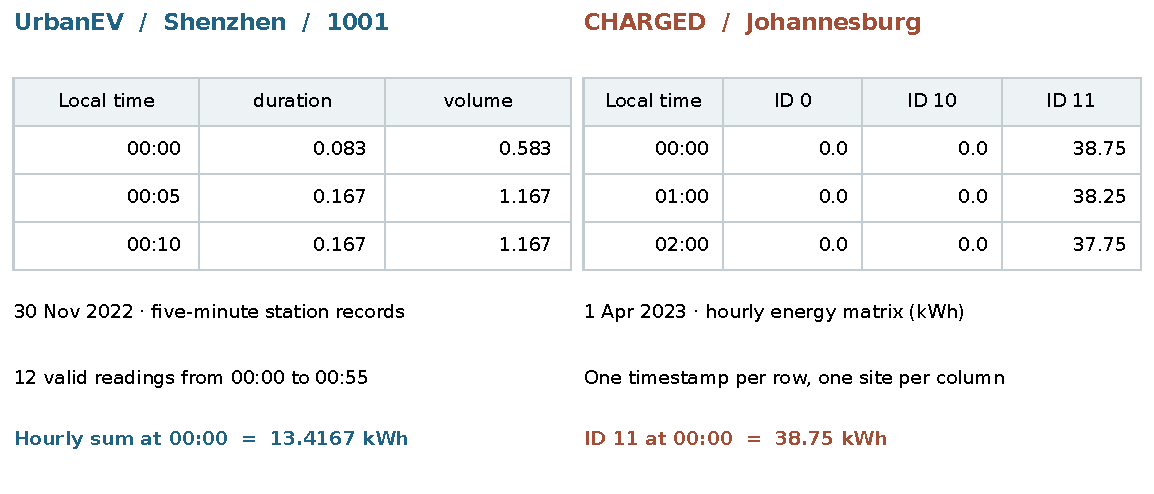
\includegraphics[width=.98\linewidth]{Images/published-records.pdf}
\caption{Published charging records and their hourly interpretation.}\label{fig:published-records}
\end{figure}

An entity key comprises dataset, city and local identifier. UrbanEV/SZH and CHARGED/SZH each have their own source population and target split. All pretraining and subsequent transfer take place within the same dataset and city. Within each group, a salted hash of the dataset, city and local identifier assigns each identifier to exactly one partition. The hash thresholds allocate approximately 60\% to Source, 20\% to Development and 20\% to Final before eligibility screening. Physical correspondence between identifiers in separate releases remains uncertain.

\section{Hourly aggregation and quality control}
For UrbanEV, the hourly total is the sum of twelve consecutive five-minute volume values. The producer requires twelve unique timestamps on the expected grid and finite, nonnegative volume and duration at each timestamp. Duration supplies a validity check. Summing a partially observed hour would systematically understate its energy, so an hour failing this check carries a missing value and a validity flag. CHARGED enters the same hourly interface directly from its released hourly matrix. Both pipelines retain the entity key, timestamp, energy in kWh and file-validity information.

\section{Partitions and target histories}
The source partition supplies established-location training examples. Table~\ref{tab:scope} counts identifiers eligible at 14 days in each partition. Readiness requires a defined entity scale. At this budget, 131 UrbanEV identifiers have undefined scales across the three partitions. To simulate cold start, each experiment restricts the history initially available at a target. The start of this history need not coincide with the opening date of the site.

\begin{table}[htbp]\centering\small
\caption{Entity inventory and eligible identifiers at 14 days.}\label{tab:scope}
\begin{tabular}{lrrrr}\toprule
 & &\multicolumn{3}{c}{Eligible identifiers}\\
\cmidrule(lr){3-5}
Group & Inventory & Source & Development & Final\\\midrule
UrbanEV/SZH &1682&914&296&341\\
CHARGED/AMS &2449&1496&475&478\\
CHARGED/JHB &47&26&8&13\\
CHARGED/LOA &229&137&51&41\\
CHARGED/MEL &63&34&14&15\\
CHARGED/SPO &47&29&8&10\\
CHARGED/SZH &1445&886&288&271\\\bottomrule
\end{tabular}\end{table}

\begin{table}[htbp]\centering\small
\caption{Target cohorts used in the reported comparisons.}\label{tab:target-cohorts}
\begin{tabular}{llrr}\toprule
Comparison & Partition & Selected IDs & History (days)\\\midrule
Backbone benchmark & Development & 4 & 14\\
Calibrated transfer comparison & Development & 12 & 7, 14, 28\\
Historical evaluation & Final & 90 & 7, 14, 28\\
Follow-up evaluation & Development & 46 & 14\\\bottomrule
\end{tabular}\end{table}

UrbanEV stations 1153, 1405, 1693 and 2152 served in both the backbone benchmark and coefficient calibration. Twelve other stations supplied the transfer comparison. The historical Final cohort included 30 UrbanEV identifiers and ten from each CHARGED group. UrbanEV identifier 2193 had no scored outcome. Crossing seven dataset--city groups with three history budgets yielded 21 comparison groups. Seeds 42, 43 and 44 repeated runs on the same entity data. Later exploratory comparisons revisited these Final outcomes.

For the follow-up comparison, the team excluded identifiers with recorded prior use, required at least one complete initial training example, and fixed the cohort before examining its outcomes. In the row order of Table~\ref{tab:scope}, the seven groups contributed 10, 10, 1, 10, 4, 1 and 10 targets. This comparison evaluates additional Development targets at 14 days. Within each group, eligible IDs were ranked by the SHA-256 hash of the study identifier, group and local ID. The first ten were selected, or all eligible IDs when fewer than ten remained. The exclusion audit covers recorded use, and the evaluation shares calendar dates with earlier experiments.

\section{From an hourly series to a forecast example}
For a target with valid observations in its permitted prefix, the energy scale is the 95th percentile of available valid hourly energy using linear interpolation. A zero percentile uses a scale of one. An empty valid prefix leaves the scale undefined and blocks forecasting. The fitted scale remains fixed through replay. For an observed hour, the energy feature is energy divided by this scale and the observation mask equals one. Missing or unavailable historical energy uses a zero placeholder with mask zero. Thus an observed zero and a missing observation produce different inputs.

The historical input has shape \(24\times7\): normalized energy, sine and cosine of local hour, sine and cosine of weekday, a weekend indicator and the energy mask. The forecast-day calendar has shape \(24\times5\) and contains only the calendar channels. An entirely missing history prevents issuance. The 24 future energy values are stored separately with their validity and availability times. A forecast can be scored and used for learning once all 24 labels have arrived and are valid. The same origins must be eligible for both methods in a paired comparison.

Figure~\ref{fig:forecast-tensors} shows the actual feature arrays for the first forecast in the example below. Hour encodings vary within each column over the day. Weekday and weekend features remain constant within each local day. On the history side, the mask stays at one even during hours of zero recorded demand.

\begin{figure}[htbp]\centering
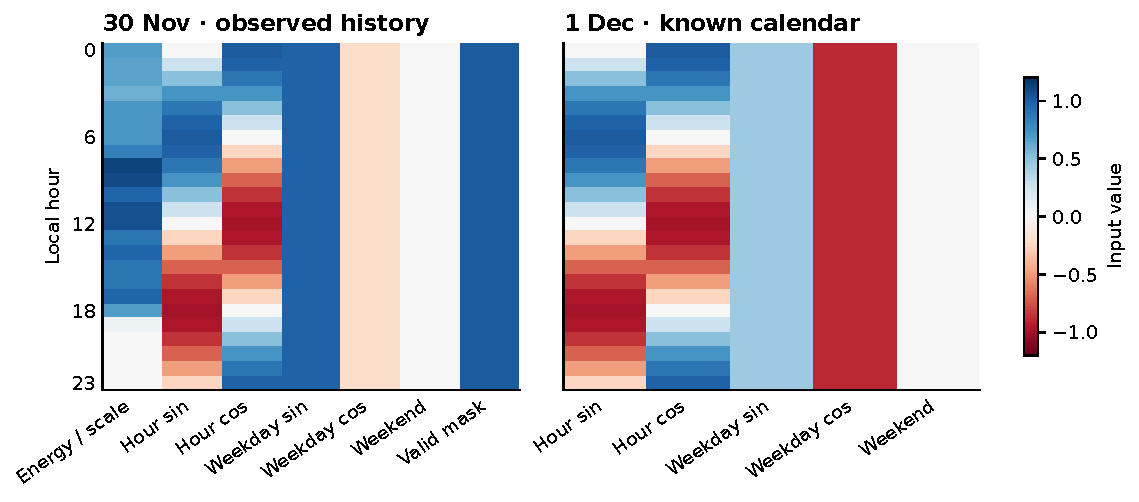
\includegraphics[width=.98\linewidth]{Images/forecast-tensors.pdf}
\caption{Feature arrays supplied to the GRU and forecast head.}\label{fig:forecast-tensors}
\end{figure}

\section{Worked example: UrbanEV station 1001}
The 14-day Development record for station 1001 begins its fit window at midnight on 17 November 2022, Shenzhen time. All 336 prefix hours are valid, including 90 observed zeros. The resulting scale is 19.9792 kWh and 13 complete initial training examples are available. Each pairs one full day of history with the following day of labels; the first pair uses 17 November to forecast 18 November and the last uses 29 November to forecast 30 November. At midnight on 1 December, the historical tensor spans 30 November and the calendar tensor describes 1 December. Figure~\ref{fig:window} displays the corresponding hourly values.



\begin{figure}[htbp]\centering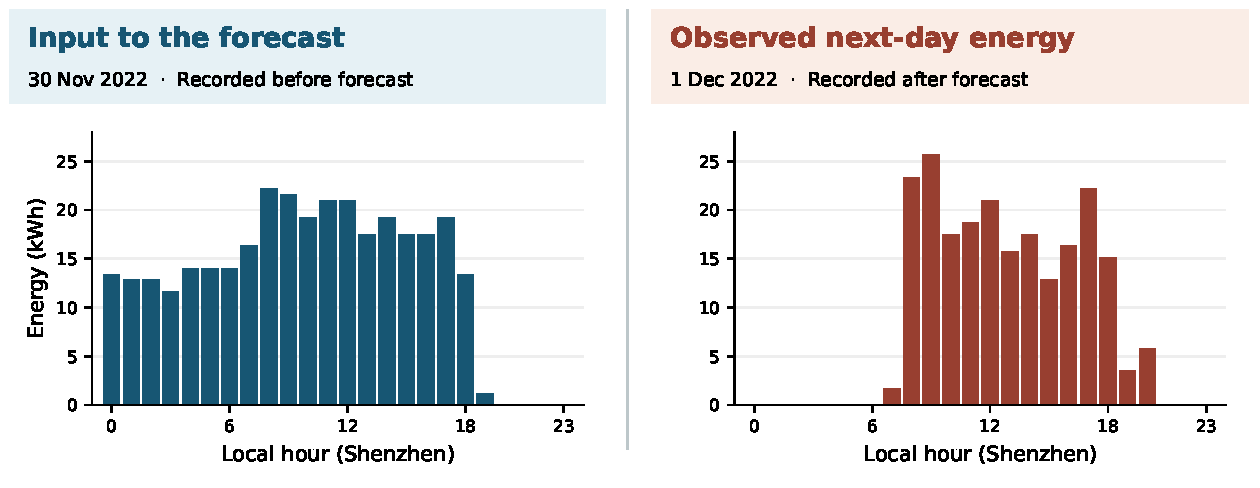
\includegraphics[width=.95\linewidth]{Images/station1001-window.pdf}
\caption{Input history and observed next-day energy at station 1001.}\label{fig:window}
\end{figure}

At 00:00 on 30 November the normalized input is 0.67153, corresponding to approximately 13.42 kWh, with mask one. The released target series on 1 December records zero energy at 06:00 and 1.75 kWh at 07:00. Both values contribute to the eventual score. The label for the final hour becomes available at midnight on 2 December under the replay clock. This example explains the timing of an input and its labels; Figure~\ref{fig:window} plots observations on both sides of the origin.

\par\penalty-200\begingroup\interlinepenalty=10000 Across the 90 requested daily origins for this identifier, 31 have entirely missing histories and 59 produce forecast inputs. Of these, 52 have complete label vectors for evaluation. Figure~\ref{fig:replay-coverage} locates these outcomes on the replay calendar, including the seven issued forecasts with incomplete labels. \par\endgroup

\begin{figure}[htbp]\centering
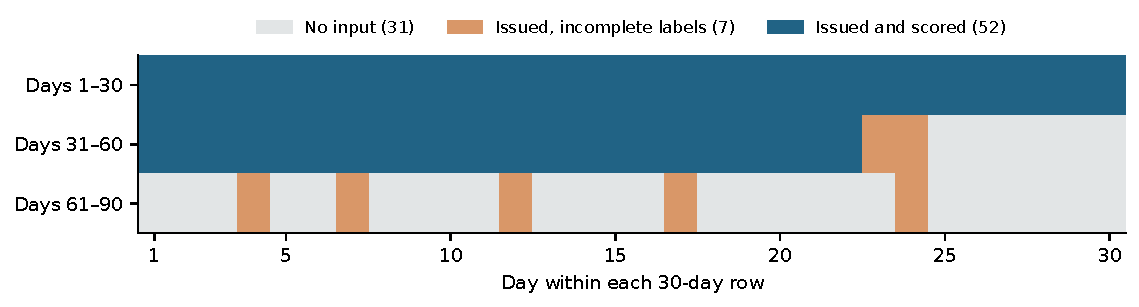
\includegraphics[width=.98\linewidth]{Images/replay-coverage.pdf}
\caption{Daily forecast availability at station 1001.}\label{fig:replay-coverage}
\end{figure}

\begin{figure}[htbp]\centering
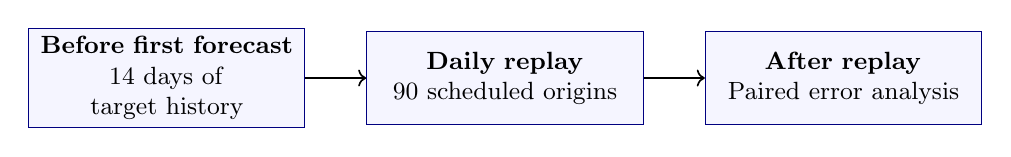
\begin{tikzpicture}[x=1cm,y=1cm]
\tikzset{stage/.style={draw=blue!50!black,fill=blue!4,align=center,text width=3.3cm,minimum height=1.18cm,inner sep=3pt,font=\small}}
\node[stage] (a) at (0,0) {\textbf{Before first forecast}\\14 days of target history};
\node[stage] (b) at (4.3,0) {\textbf{Daily replay}\\90 scheduled origins};
\node[stage] (c) at (8.6,0) {\textbf{After replay}\\Paired error analysis};
\draw[->,semithick](a.east)--(b.west);
\draw[->,semithick](b.east)--(c.west);
\end{tikzpicture}
\caption{Timeline for the locked 46-target evaluation.}\label{fig:locked-timeline}
\end{figure}

In Figure~\ref{fig:locked-timeline}, forecasts precede the next day's observations. The paired analysis uses seven-day calendar blocks, with three- and fourteen-day sensitivity checks. All 36 CHARGED targets had 90 scored days. UrbanEV coverage ranged from 51 to 90 days. Each target mean describes its observed days; the cause of missing observations is unknown.

\usetikzlibrary{arrows.meta,positioning}
\chapter{Methodology}
\label{chap:methodology}
At each local midnight, the forecaster estimates the next 24 hourly energy values at a target charging location. With only a short history at that location, the model can start from weights learned at other locations in the same dataset and city. We examine two subsequent decisions. During training, how strongly should the target encoder be constrained to preserve the source representation? At forecast time, how much weight should each of two adaptation trajectories receive?

\section{Forecasting workflow}
We train the source model on eligible historical windows from source identifiers. Each dataset--city group and random seed has its own checkpoint. In the historical study, seven groups and three seeds yield 21 source checkpoints. For each target identifier, history budget and seed, adaptation starts separately from the corresponding checkpoint. With no complete examples in the target prefix, initial adaptation performs zero optimizer steps.

Figure~\ref{fig:ch4fusion} follows one forecast from the pretrained forecaster through two target models. Both models use the same target history and future calendar. Once the actual demand arrives, the stored forecasts supply the errors for the next weight update. Section~\ref{sec:retention} describes the earlier experiment that deploys a single branch at a time.

\begin{figure}[htbp]\centering
\resizebox{\linewidth}{!}{\definecolor{evBlue}{HTML}{205B82}
\definecolor{evRust}{HTML}{A74731}
\begingroup\def\baselinestretch{1}
\begin{tikzpicture}[x=1cm,y=1.55cm,>=Latex,
 box/.style={draw=evBlue!65,fill=evBlue!4,rounded corners=2pt,text width=4.10cm,align=center,inner sep=5pt,minimum height=1.18cm,font=\small},
 warm/.style={box,draw=evRust!65,fill=evRust!4},
 pathline/.style={->,draw=black!70,line width=.65pt},
 lab/.style={font=\scriptsize,fill=white,inner sep=2pt}]
\node[box] (src) at (0,3.9) {\textbf{Source training}\\Established sites\\GRU encoder and forecast head};
\node[box] (init) at (5.3,3.9) {\textbf{Target adaptation}\\Source initialization\\(7, 14 or 28 days initially)};
\draw[pathline] (src)--(init);
\node[box] (input) at (10.6,3.9) {\textbf{Each forecast origin}\\Previous 24 hours ($24\times7$)\\Next-day calendar ($24\times5$)};
\node[box] (st) at (2.65,1.50) {\textbf{Stable GRU}\\$F+R$, frozen source reference\\Train on the newly arrived day};
\node[warm] (fa) at (7.95,1.50) {\textbf{Fast GRU}\\$F$, no retention penalty\\Train on up to seven recent days};
\coordinate (shared) at (5.3,2.65);
\draw[draw=black!70,line width=.65pt] (init.south)--(shared);
\draw[draw=black!70,line width=.65pt] (input.south) |- (shared);
\fill[black!70] (shared) circle (1.3pt);
\draw[pathline] (shared)--++(0,-.22) -| (st.north);
\draw[pathline] (shared)--++(0,-.22) -| (fa.north);
\node[box] (mix) at (5.3,-.70) {\textbf{Issue 24 hourly estimates}\\$\hat y_t=w_t\hat y_{S,t}+(1-w_t)\hat y_{F,t}$};
\draw[pathline] (st.south) |- ([yshift=2pt]mix.west);
\draw[pathline] (fa.south) |- ([yshift=2pt]mix.east);
\node[box] (score) at (5.3,-2.65) {\textbf{Score the saved expert forecasts}\\24 labels arrive\\Compute normalized daily MAE};
\draw[pathline] (mix)--(score);
\node[warm] (next) at (10.6,-2.65) {\textbf{Next forecast weight}\\Update with expert losses\\$w^+=0.1+0.8p$};
\draw[pathline] (score)--(next);
\draw[pathline,draw=evRust] (next.north) |- ([yshift=-4pt]mix.east);
\end{tikzpicture}\endgroup
}
\caption{Source initialization, target adaptation and forecast fusion.}\label{fig:ch4fusion}
\end{figure}

\section{GRU encoder and training objective}
The input window contains 24 hourly vectors with seven features each. The prediction head also receives five known calendar features for each future hour. A standard gated recurrent unit (GRU) encodes the history \cite{cho2014}. The encoder has two layers of width 64, zero dropout and a fresh hidden state for each window.

The last-layer final state $h_{24}\in\mathbb R^{64}$ is concatenated with the 120 flattened future-calendar values. The head applies a width-64 linear layer, ReLU, a 24-output linear layer and Softplus. The primary forecaster has 52,376 trainable parameters.


Figure~\ref{fig:gru-forward} follows the two inputs through a single forecaster. The calendar enters after the history has been encoded. During target training, the same 64-dimensional history representation also enters the retention penalty.
\begin{figure}[htbp]\centering
\resizebox{.95\linewidth}{!}{\begingroup\def\baselinestretch{1}
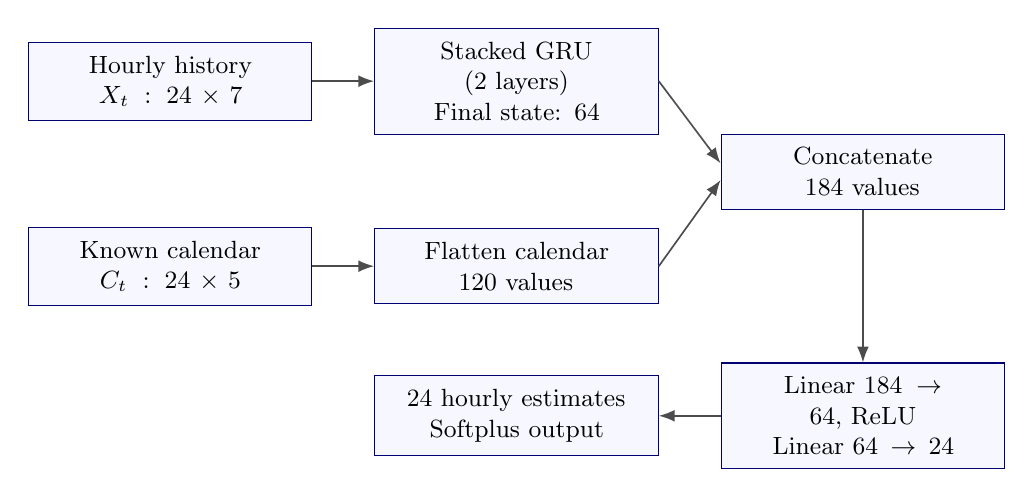
\begin{tikzpicture}[x=1cm,y=1cm,>=Latex,
 box/.style={draw=blue!45!black,fill=blue!3,align=center,text width=3.25cm,inner sep=5pt,font=\small},
 a/.style={->,semithick,draw=black!70}]
\node[box] (x) at (0,0) {Hourly history\\$X_t:24\times7$};
\node[box] (c) at (0,-2.35) {Known calendar\\$C_t:24\times5$};
\node[box] (h) at (4.4,0) {Stacked GRU (2 layers)\\Final state: 64};
\node[box] (f) at (4.4,-2.35) {Flatten calendar\\120 values};
\node[box] (cat) at (8.8,-1.15) {Concatenate\\184 values};
\node[box] (out) at (4.4,-4.25) {24 hourly estimates\\Softplus output};
\node[box] (head) at (8.8,-4.25) {Linear $184\to64$, ReLU\\Linear $64\to24$};
\draw[a](x)--(h);\draw[a](c)--(f);\draw[a](h.east)--([yshift=3pt]cat.west);
\draw[a](f.east)--([yshift=-3pt]cat.west);
\draw[a](cat.south)--(head.north);
\draw[a](head)--(out);
\end{tikzpicture}\endgroup
}
\caption{History encoder and calendar-conditioned forecast head.}\label{fig:gru-forward}
\end{figure}

\subsection{Forecast loss and latent retention}

Li et al.~\cite{li2018} use pretrained parameters as the reference for an explicit transfer penalty. Here we use the frozen source encoder as a reference in representation space and scale each coordinate by its source variability. The target GRU minimizes a forecast error $F_B$ and a latent penalty $R_B$ over a batch $B$ of complete days. For example $j$ and forecast hour $q$, $\widetilde y$ and $\widehat{\widetilde y}$ denote observed and predicted energy normalized by the target scale.
\begin{equation}\begin{aligned}
L_B(\theta,\lambda)&=F_B(\theta)+\lambda R_B(\theta),\\
F_B(\theta)&=\frac{1}{24|B|}\sum_{j\in B}\sum_{q=1}^{24}
|\widehat{\widetilde y}_{j,q}(\theta)-\widetilde y_{j,q}|,\\
R_B(\theta)&=\frac{1}{64|B|}\sum_{j\in B}\sum_{k=1}^{64}
\left(\frac{h_k(x_j;\theta)-h_k(x_j;\theta_s)}{s_k+0.001}\right)^2 .
\end{aligned}\label{eq:total}\end{equation}
In Equation~\eqref{eq:total}, both encoders process the same target history $x_j$. The source parameters $\theta_s$ and population standard deviation (computed over source training encodings) $s_k$ of each latent coordinate stay fixed. Adam updates the target parameters $\theta$. A positive $\lambda$ penalizes divergence from the source encoding. At $\lambda=0$, the target learns from forecast error alone and retains its source initialization.

\section{Fixed retention and coefficient calibration}
Historical fixed retention uses a constant $\lambda=1$. The original selector considers $\{0,0.1,1\}$ and starts from a common target adaptation at $\lambda=0.1$. These coefficients define the historical comparison. Their effective penalty strength depends on the gradients measured during target training.

The twelve-entity Development study uses independent trajectories at the same three coefficients but selects its Fixed comparator on the four calibration entities. It selects $\lambda=1,1,0$ for 7-, 14- and 28-day prefixes. Thus its Fixed row is not identical to the historical fixed-one recipe. A zero coefficient in that row still retains Source initialization.

\subsection{Expanded fixed-coefficient diagnostic}
The four-target coefficient study evaluates 21 real coefficients, including zero, using a finite Gaussian-process/expected-improvement search on positive log coefficients plus a coverage sensitivity grid. Acquisition is maximized approximately on 4,097 numeric grid points. Calibration averages forecast MAE equally across entities and paired seeds on the first 28 scheduled origins:
\begin{equation}
\lambda^*=\underset{\lambda\in\Lambda_{\rm measured}}{\operatorname{argmin}}\;
\frac{1}{4}\sum_{i=1}^4\frac{1}{3}\sum_{s=42}^{44}
\operatorname{MAE}^{\rm Cal}_{i,s}(\lambda).
\label{eq:fixedselection}
\end{equation}
The positive search interval is derived from prefix-only gradient-balance coefficients after three unregularized target epochs: its lower endpoint is 0.01 times the minimum measured balance coefficient, and its upper endpoint is 100 times the maximum. These factors deliberately span weak to dominant local penalty gradients; they are engineering coverage choices. Zero is evaluated separately. The resulting positive search interval was $[0.00038785,33.84425]$. The best measured coefficient lay inside the interval. Exact ties in calibration MAE favour the smaller coefficient. The search follows the Gaussian-process approach to hyperparameter optimization \cite{snoek2012}.
Equation~\eqref{eq:fixedselection} selected $\lambda^*=0.798445$ among the measured candidates. Chapter~5 reports the measured gradient ratios and forecast errors for representative coefficients.

\section{Adaptive retention mechanisms}\label{sec:retention}
\subsection{Confidence-gated block selection}
\begin{figure}[htbp]
\centering\resizebox{.96\linewidth}{!}{\definecolor{FlowBlue}{HTML}{2166AC}
\definecolor{FlowRed}{HTML}{B2182B}
\begin{tikzpicture}[x=1cm,y=1cm,>=Latex,every node/.style={font=\footnotesize,align=center},
box/.style={draw=black!40,rounded corners=2pt,fill=white,inner sep=6pt,text width=3.5cm,minimum height=1.1cm},
flow/.style={->,draw=black!65,line width=.7pt}]
\node[box,fill=FlowBlue!7,draw=FlowBlue!65] (start) at (0,0) {\textbf{Selected trained state}\\Model and Adam moments};
\node[box,fill=FlowBlue!7,draw=FlowBlue!65] (fork) at (5.2,0) {\textbf{Clone at block start}\\$\lambda\in\{0,0.1,1\}$};
\node[box] (pred) at (10.4,0) {\textbf{Predict and learn}\\Three causal branches};
\node[box] (labels) at (10.4,-2.8) {\textbf{Complete arrived errors}\\Paired within the 14-day block};
\node[box,fill=FlowRed!6,draw=FlowRed!65] (decision) at (5.2,-2.8) {\textbf{Bootstrap lower bounds}\\$n\ge7$ paired days\\Switch only if $L_c>0$};
\node[box,fill=FlowBlue!7,draw=FlowBlue!65] (carry) at (0,-2.8) {\textbf{Carry selected branch}\\Keep its trained model and Adam};
\draw[flow] (start)--(fork);\draw[flow] (fork)--(pred);\draw[flow] (pred)--(labels);
\draw[flow] (labels)--(decision);\draw[flow] (decision)--(carry);\draw[flow] (carry)--(start);
\end{tikzpicture}
}
\caption{Historical confidence-guided retention selection.}\label{fig:retention}
\end{figure}
Figure~\ref{fig:retention} shows the original retention controller. It begins each 14-day block by cloning the selected model and Adam state into three branches, one per retention coefficient. All branches forecast causally and train on the same eligible data. Only the active branch supplies the deployed forecast. At the next boundary, complete arrived daily errors within the block are paired.

We use moving-block resampling for dependent observations \cite{kunsch1989}. Our switching rule compares the errors of challenger $c$ and active branch $a$ on the same completed day $d$. We define
\begin{equation}\begin{aligned}
D_{c,d}&=e_{a,d}-e_{c,d},\\
L_c&=Q_{0.025}\!\left(\overline{D}_{c}^{*(1)},\ldots,
\overline{D}_{c}^{*(2000)}\right).
\end{aligned}\label{eq:lcb}\end{equation}
Positive differences favor the challenger. Resamples concatenate noncircular overlapping segments of three chronological valid daily observations, trimming to the original valid-day count. Both challengers use identical sampled indices. The 0.025 tail implements the specified two-challenger adjustment with interval parameter 0.05. Quantiles are linearly interpolated.

If fewer than seven complete days are available, or no challenger has $L_c>0$, the active branch is retained. Otherwise the controller selects the greatest qualifying lower bound, breaking exact ties by proximity to the current coefficient and then ascending coefficient order. The selected \emph{trained} model and optimizer continue forward, and are cloned again at the new block start. Keeping the active branch does not restore its block-start weights.

Algorithm~\ref{alg:retention} gives the order of forecasting, learning and branch selection. The lower bound describes differences observed in the completed block. Missing days compress the sequence used for resampling.

\begin{algorithm}[htbp]
\caption{Retention selection at a target station}\label{alg:retention}
\begin{algorithmic}[1]
\State Initialize the target from source and adapt on the eligible prefix at $\lambda=0.1$.
\For{each 14-day block}
  \State Copy the active model and Adam state to branches with $\lambda\in\{0,0.1,1\}$.
  \For{each forecast origin in the block}
    \State Update each branch on eligible earlier feedback and save its new forecast.
    \State Issue the forecast from the active branch.
  \EndFor
  \State At the boundary, process eligible arrivals and pair complete daily errors.
  \If{at least seven paired days are available}
    \State Compute challenger bounds using Equation~\eqref{eq:lcb}.
    \State Select the highest positive bound if one exists, using the tie rule above.
  \EndIf
  \State Carry the selected trained model and its Adam state into the next block.
\EndFor
\end{algorithmic}
\end{algorithm}

\subsection{Common-bank online selection}
The separate twelve-entity study trains independent constant-coefficient trajectories instead of reforking a chosen state every block. Its past-MAE selector and confidence selector choose outputs from this same bank, starting from the calibration-selected Fixed trajectory. Both rules nominate the candidate with the lowest past MAE. The confidence variant gates that same nomination before switching. It uses seven-day blocks, at least five complete days, segment length three, 2,000 resamples and the same zero-margin principle.

This matched bank compares two output-selection rules. It is not a rerun of the original 14-day model-reforking procedure. 

A separate four-target study tested a continuous coefficient. It used two earlier days for a virtual training step and a more recent observed day to estimate how changing $\lambda$ would affect forecast error. Appendix~\ref{app:continuous} gives the update and calibration settings. A further calibration experiment tested a shadow model and transferred its proposed coefficient only after sufficient paired evidence.


Figure~\ref{fig:continuous-step} shows one eligible update of the continuous controller. The virtual step changes a temporary copy of the parameters. The validation gradient determines the coefficient used by the real optimizer when the newly arrived example enters training.
\begin{figure}[htbp]\centering
\resizebox{.95\linewidth}{!}{\begingroup\def\baselinestretch{1}
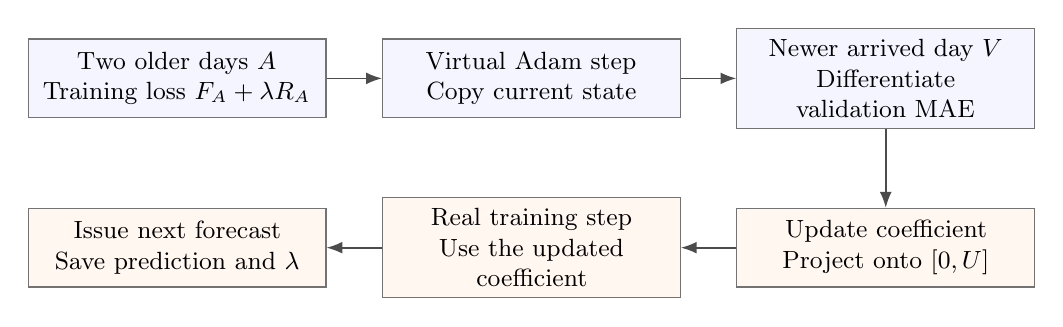
\begin{tikzpicture}[x=1cm,y=1cm,>=Latex,
 box/.style={draw=black!55,align=center,text width=3.5cm,minimum height=1.0cm,inner sep=4pt,font=\small},
 a/.style={->,semithick,draw=black!70}]
\node[box,fill=blue!4] (a) at (0,0) {Two older days $A$\\Training loss $F_A+\lambda R_A$};
\node[box,fill=blue!4] (v) at (4.5,0) {Virtual Adam step\\Copy current state};
\node[box,fill=blue!4] (g) at (9,0) {Newer arrived day $V$\\Differentiate validation MAE};
\node[box,fill=orange!6] (lambda) at (9,-2.15) {Update coefficient\\Project onto $[0,U]$};
\node[box,fill=orange!6] (real) at (4.5,-2.15) {Real training step\\Use the updated coefficient};
\node[box,fill=orange!6] (issue) at (0,-2.15) {Issue next forecast\\Save prediction and $\lambda$};
\draw[a](a)--(v);\draw[a](v)--(g);\draw[a](g)--(lambda);\draw[a](lambda)--(real);\draw[a](real)--(issue);
\end{tikzpicture}\endgroup
}
\caption{Virtual and real updates in the continuous retention experiment.}\label{fig:continuous-step}
\end{figure}

\section{Adaptive fusion of two retention experts}
\subsection{Complementary trajectories}


The fusion extension in Figure~\ref{fig:ch4fusion} retains two GRUs initialized from the source checkpoint at epoch 10. The stable expert is the historical Fixed model: $\lambda_S=1$, three initial target epochs when complete prefix examples exist, learning rate 0.001, and one online epoch on each newly arrived complete daily example. The historical comparison reuses the forecasts previously issued by this model.

The fast expert uses $\lambda_F=0$, the same three initial epochs and learning rate, and one online epoch over available complete examples in the seven calendar days ending at the arrived example's forecast origin. The window may include permitted prefix examples, contains at most seven complete daily examples, and fits one optimizer step. It never includes labels that have not arrived.

The experts differ in both retention and update memory. A gain from combining them therefore cannot be attributed solely to different coefficients. Both start from Source; the fast expert is not target-only. Their coefficients remain constant throughout fusion.

\subsection{Weight update}
For stable weight $w_t$, the issued 24-hour forecast is
\begin{equation}
\hat y_{t,q}=w_t\hat y_{S,t,q}+(1-w_t)\hat y_{F,t,q}.
\label{eq:fusion}\end{equation}
Once all 24 labels for an earlier day $d$ arrive, each expert's loss $\ell_{e,d}$ is its mean absolute hourly error in kWh divided by the target energy scale $c_i$. Both losses use the forecasts stored at issue time.
At feedback event $k$, we apply the two-expert Fixed-share update of Herbster and Warmuth \cite{herbster1998} to the normalized daily losses. The resulting weight applies to subsequent forecasts.
\begin{equation}\begin{aligned}
p_k&=\frac{w_k\exp(-\eta\ell_{S,d})}
{w_k\exp(-\eta\ell_{S,d})+(1-w_k)\exp(-\eta\ell_{F,d})},\\
w_{k+1}&=(1-\alpha)p_k+\alpha(1-p_k)\\
&=\alpha+(1-2\alpha)p_k.
\end{aligned}\label{eq:fixedshare}\end{equation}
The implementation uses equivalent log-odds arithmetic. Calibration selects $w_0=0.430782$, $\eta=0.1$ and $\alpha=0.1$. Updated weights consequently lie in $[0.1,0.9]$. This bound follows from sharing, not from a lambda search. No complete feedback means no weight update; elapsed time alone does not decay the weight.

The weight at forecast origin $t$ is the state after all eligible feedback events $k$ preceding issuance have been processed. The runner applies Equation~\eqref{eq:fixedshare} to earlier feedback before issuing the current forecast with Equation~\eqref{eq:fusion}. Both experts continue training under their respective fixed retention coefficients.

\subsection{Calibration and matched fusion controls}
Four calibration entities and seeds 42--44 compare fast windows of 3, 7 and 14 days with learning rates 0.001 and 0.003. For each pair, a static stable weight minimizes equal-cell Calibration MAE on $[0,1]$ via the weighted-median solution of the convex absolute-error objective. This selects the seven-day, 0.001 recipe and the initial weight above.

Nine weight-controller candidates cross $\eta\in\{0.1,1,10\}$ and $\alpha\in\{0.001,0.01,0.1\}$. Calibration selects the final settings before their historical full-scope comparison. The same recipe is carried to all namespaces and histories without per-namespace recalibration. These bounded engineering grids do not establish global optimality.

The decisive control is static fusion with the same stable and fast forecasts and fixed $w_0$. Fast-only tests one component. Equal 50/50 fusion and loss-free sharing are posthoc diagnostics; in loss-free sharing, the posterior equals the prior before the same share step. This retains attraction toward one-half while removing the expert-loss signal.

\section{Training setup and evaluation}
\subsection{Implementation and hyperparameters}
The 46-target Development evaluation ran in Python 3.12.13 with PyTorch 2.11.0. Table~\ref{tab:ch4training} gives its locked training settings. Each seed identifies the source checkpoint and pairs the methods evaluated on the same target and forecast origins.

\begin{table}[htbp]\centering\small
\caption{Training settings for the 46-target evaluation.}\label{tab:ch4training}
\begin{tabular}{ll}\toprule
Setting & Value\\\midrule
Source checkpoint & Epoch 10 within each dataset--city group\\
Initial target history & 14 days\\
Optimizer, learning rate, batch size & Adam, 0.001, 64\\
Initial target training & 3 epochs on complete prefix examples\\
Online training & 1 epoch per complete arrival\\
Stable and fast retention & $\lambda_S=1$, $\lambda_F=0$\\
Fast update window & 7 calendar days\\
Fusion settings & $w_0=0.430782$ (rounded), $\eta=\alpha=0.1$\\
Paired seeds & 42, 43, 44\\\bottomrule
\end{tabular}\end{table}
\subsection{Baseline and training-budget controls}
Each implementation has 172 unique model--mode--entity--seed records: 160 nonspatial and 12 spatial; deterministic methods have no artificial seed replicates. Nonspatial neural models use three Source epochs, three target epochs (batch four; learning rate 0.0005), and one online epoch per eligible arrival. GCN--LSTM instead uses five initial epochs, learning rate 0.001 and single-example steps. Classical methods have separate fitting and refitting rules. The \href{https://github.com/HungLD9505/adaptive-retention-ev/tree/52a91d3/docs/reports/issue99-teacher-review-20261111}{benchmark archive} identifies the executed versions and score tables for implementations A and B. The export from A lacks issuance timestamps for individual scores, which limits independent verification of their timing.

The subsequent GRU study reuses Source epoch 10 and calibrates initial target epochs over $\{3,10,30,100,300\}$. The objective uses the first 28 scheduled origins of the four calibration entities, with equal entity and seed weights. The declared extension to 900 epochs is unused because no 300-epoch candidate wins. Target-only selects 30/100/100 epochs across 7/14/28 days; Source-initialized models select 3/3/10. The learning rate is 0.001. The twelve additional entities then evaluate these recipes.

\subsection{Daily replay and evaluation}
For the station 1001 example in Chapter~3, the midnight forecast on 1 December uses the observed history for 30 November and the calendar for 1 December. The last hourly label for 1 December arrives at midnight on 2 December. Only then can the full daily vector contribute an error for that forecast. At each origin the runner first processes complete earlier arrivals, ordered by availability and then by forecast origin, applies any due decision, and stores the new forecast. Missing target labels remain missing.

The primary error for one complete day is the mean absolute difference across its 24 hourly values in kWh. For the follow-up evaluation, methods are compared on matched origins. The analysis first averages over paired seeds and scored entities within each dataset--city group, computes the percentage MAE reduction relative to each control, then averages reductions equally over the seven groups. This gives a small group the same weight as a large group. Seeds repeat training on the same entity records.

The historical comparisons cover three initial histories on previously inspected targets. The follow-up fixes the target list, both controls and the decision criterion before examining the selected outcomes. It uses 46 additional Development identifiers, 14 days of initial history, three seeds and 90 scheduled origins per target and seed. The primary uncertainty analysis uses 10,000 paired resamples. Within each group, it resamples target IDs and draws circular seven-day calendar blocks shared across the sampled IDs and both comparisons. The paired seeds are averaged before resampling. Allocating a family error level of 0.05 equally to two comparisons gives nominal 97.5\% percentile intervals. Any replicate with an undefined statistic makes the corresponding interval undefined. In this evaluation each expert forecast was saved before its labels arrived; the mixture was evaluated in a causal replay of the saved forecasts and delayed feedback. The prespecified criterion requires a scored outcome for every selected target and positive lower interval endpoints against both single Fixed and matched static fusion. Chapter~5 reports the estimates and intervals for those comparisons.

\chapter{Results Analysis}\label{chap:results}
\section{Evaluation scope}
The experiments address three decisions at a charging location with limited history. The first is whether to initialize a forecaster from other locations. The second is how strongly to constrain the target encoder during adaptation. The third is whether to vary the contribution of two forecasters after observing their errors. Table~\ref{tab:res-scope} identifies the targets and comparison used for each decision.

\begin{table}[H]\centering\small
\caption{Target populations and initial histories.}\label{tab:res-scope}
\begin{tabular}{>{\raggedright\arraybackslash}p{.29\linewidth}>{\raggedright\arraybackslash}p{.36\linewidth}l}\toprule
Comparison & Target identifiers & History (days)\\\midrule
Backbone benchmark & 4 UrbanEV Development & 14\\
GRU initialization & 12 additional UrbanEV Development & 7, 14, 28\\
Coefficient calibration & 4 UrbanEV Development & 14\\
Historical selection and fusion & 90 selected across 7 dataset--city groups, Final partition & 7, 14, 28\\
Follow-up fusion evaluation & 46 additional Development IDs across 7 groups & 14\\
\bottomrule\end{tabular}
\end{table}

MAE measures the absolute error in hourly energy, in kWh. Lower values indicate better forecasts. Within a comparison, methods are scored on matched forecast origins with complete next-day observations. The historical comparison contains 21 groups from seven dataset--city groups crossed with three history budgets. One of the 90 selected identifiers had no scored outcome. Repeated seeds share target observations. The historical cohort was revisited during method development. The final comparison in this chapter uses a separately locked list of Development identifiers.

\clearpage
\section{Source transfer and backbone choice}
\subsection{Independent backbone benchmarks}
Two implementations evaluated models on the same four UrbanEV targets with 14 days of initial history. Table~\ref{tab:baselines} gives the mean error in each training mode. Bold marks the lowest MAE in each column. A dash denotes a mode without a reported result. Custom attention in A and official TimeXer in B \cite{wang2024timexer} are distinct architectures. The separate spatial benchmark uses histories from supporting locations. Its MAE is reported once per implementation.
\begin{table}[H]
\centering\small
\caption{Independent baseline MAE on four UrbanEV targets (kWh).}\label{tab:baselines}
\begin{tabular*}{\textwidth}{@{\extracolsep{\fill}}lrrrr@{}}\toprule
& \multicolumn{2}{c}{Implementation A} & \multicolumn{2}{c}{Implementation B}\\\cmidrule(lr){2-3}\cmidrule(l){4-5}
Model & Target only & Transfer & Target only & Transfer\\\midrule
Daily naive & 7.0763 & -- & 7.0757 & --\\
Weekly naive & 8.4631 & -- & 8.4631 & --\\
Ridge & 5.9339 & -- & 5.9339 & --\\
SARIMA & 6.5799 & -- & 6.6771 & --\\
Random forest & \textbf{5.8008} & -- & \textbf{5.8204} & --\\
XGBoost & 6.4847 & -- & 6.4613 & --\\
MLP & 8.6711 & 5.5196 & 8.6855 & 5.4753\\
GRU & 8.9406 & \textbf{5.3150} & 8.9239 & 5.3157\\
LSTM & 8.9360 & 5.3356 & 8.9565 & 5.3168\\
TCN & 8.0734 & 5.3447 & 7.8415 & 5.3027\\
Custom attention & 8.1209 & 5.5823 & -- & --\\
Official TimeXer & -- & -- & 7.0224 & \textbf{5.1979}\\
\midrule
GCN--LSTM (spatial) & \multicolumn{2}{c}{7.1288} & \multicolumn{2}{c}{7.1790}\\
\bottomrule\end{tabular*}
\end{table}

Random forest had the lowest target-only MAE in both implementations. With source initialization, GRU ranked first in A (5.3150 kWh), narrowly ahead of LSTM (5.3356). In B, TimeXer ranked first (5.1979), followed by TCN (5.3027) and GRU (5.3157). Across both implementations, all 60 paired neural model--entity--seed comparisons per implementation favored source initialization. The GRU provided a competitive backbone with 52,376 trainable parameters for the controlled retention experiments. The ranking applies to the training settings and four targets tested here.

\subsection{Transfer after calibrating the target training budget}
A target-only neural model may need more initial training than a pretrained one. We compared 3, 10, 30, 100 and 300 initial epochs on four calibration targets. The lowest calibration MAE occurred at 30, 100 and 100 epochs for target-only training with 7, 14 and 28 days of history, respectively. With source initialization, the corresponding values were 3, 3 and 10 epochs. We evaluated these settings on twelve additional targets. Both models used the same architecture and scored days. Source fine-tuning used zero latent penalty, so the comparison measures the benefit of starting from a source checkpoint under the separately calibrated budgets.


Figure~\ref{fig:budget-curves} shows why the two initialization modes received different training budgets. Open circles mark the lowest calibration MAE on each curve. Table~\ref{tab:res-transfer} reports the subsequent evaluation on twelve additional targets.
\begin{figure}[htbp]\centering
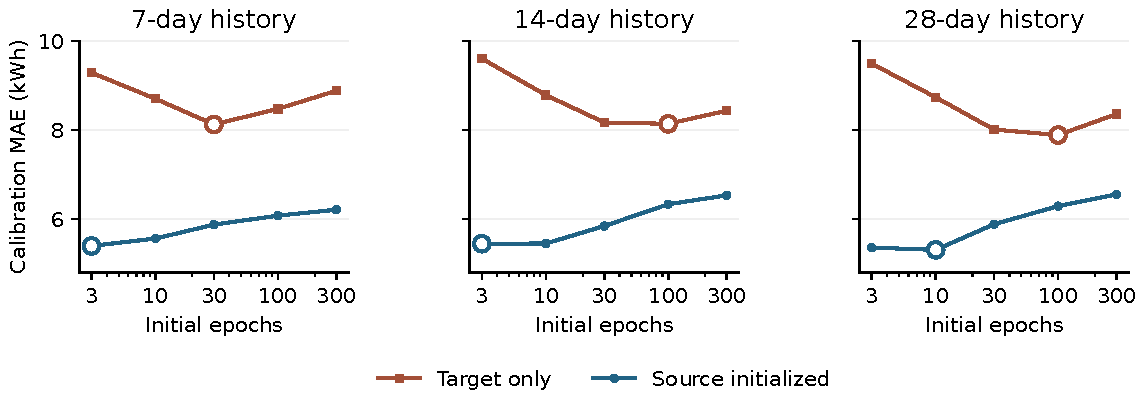
\includegraphics[width=.97\linewidth]{Images/budget-curves.pdf}
\caption{Initial training budget on four calibration targets.}\label{fig:budget-curves}
\end{figure}

\begin{table}[H]\centering\small
\caption{GRU initialization on twelve UrbanEV targets (MAE in kWh).}\label{tab:res-transfer}
\begin{tabular}{lrrr}\toprule
Initial history & Target-only MAE & Transfer MAE & Reduction\\\midrule
7 days & 5.0521 & \textbf{3.3671} & 33.35\%\\
14 days & 4.8341 & \textbf{3.3046} & 31.64\%\\
28 days & 4.7697 & \textbf{3.3482} & 29.80\%\\
\bottomrule\end{tabular}
\end{table}

At 14 days, for example, source initialization reduced mean error by 1.5295 kWh per hour (Table~\ref{tab:res-transfer}). The advantage persisted at 28 days despite allowing the target-only model 100 initial epochs. These reductions describe the mean over the selected UrbanEV targets at each budget. They provide a reason to retain source initialization when studying the smaller effects of regularization and online decisions. The four-target backbone benchmark also used a different source training budget (three epochs versus ten here), so its absolute MAEs should be interpreted within that benchmark.
\clearpage
\section{Fixed and adaptive retention}
\subsection{Measured retention strength on the calibration targets}
For each tested coefficient, the encoder gradient ratio compares the weighted retention gradient with the forecast gradient on the same parameters,
\begin{equation}
\rho=\frac{\|\lambda\nabla_{\theta_{\rm enc}}R\|_2}{\|\nabla_{\theta_{\rm enc}}F\|_2+10^{-12}}.
\end{equation}
\begin{table}[H]\centering
\caption{Representative fixed coefficients on four calibration targets.}
\small\begin{tabular}{lrrr}\toprule
Role & $\lambda$ & Median $\rho$ & MAE (kWh)\\\midrule
Zero reference & 0 & 0 & 5.443630\\
Forecast-dominated, higher MAE & 0.000390 & 0.000922 & 5.444004\\
Forecast-dominated, lower MAE & 0.474980 & 0.559958 & 5.361266\\
Calibration minimum & 0.798445 & 0.792279 & \textbf{5.331706}\\
Retention-dominated, lower MAE & 8.163598 & 7.234187 & 5.371132\\\bottomrule
\end{tabular}
\end{table}
Among the twenty positive coefficients, five had a median gradient ratio below one and a higher calibration MAE than zero retention. Ten had a ratio below one and a lower MAE. The other five had a ratio above one and a lower MAE. Each representative row illustrates an observed combination of gradient strength and error direction relative to zero. These classifications apply at the sampled points. The calibration minimum is shown separately.

\begin{figure}[H]\centering
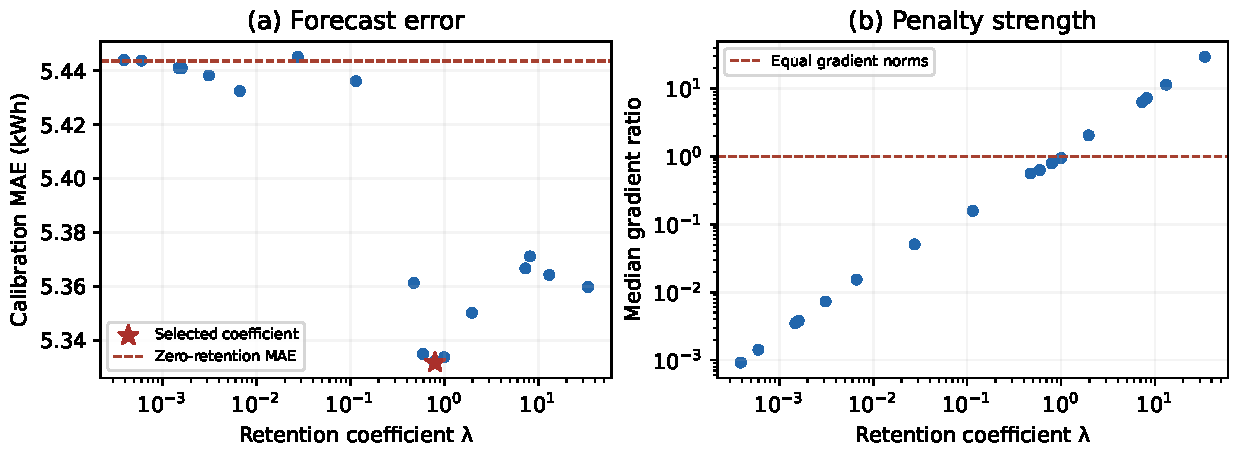
\includegraphics[width=.95\linewidth]{Images/fixed-evidence.pdf}
\caption{Calibration error and encoder gradient ratios.}\label{fig:res-fixed}\end{figure}

Figure~\ref{fig:res-fixed} plots the 20 positive coefficients on a logarithmic axis. The dashed lines mark zero-retention MAE in (a) and equal gradient norms in (b). The selected coefficient reduced calibration MAE by 0.111925 kWh.

\subsection{Does switching retention reduce forecast error?}
The historical selector could switch among three coefficients after a completed block. The candidates used $\lambda\in\{0,0.1,1\}$. Its comparator held $\lambda=1$. Figure~\ref{fig:res-selector} compares the percentage reduction in group MAE against Fixed and Online-best. Positive values favor switching. Against Fixed, all three histories favored switching in CHARGED/MEL, SPO and SZH, giving nine wins. All three favored Fixed in UrbanEV/SZH, AMS, JHB and LOA. Against Online-best, which selects by past error without a confidence gate, the historical confidence rule yielded lower MAE in eleven of 21 groups. In each comparison all eighteen finite exploratory intervals included zero. The three UrbanEV intervals were undefined in each comparison.

\begin{figure}[H]\centering
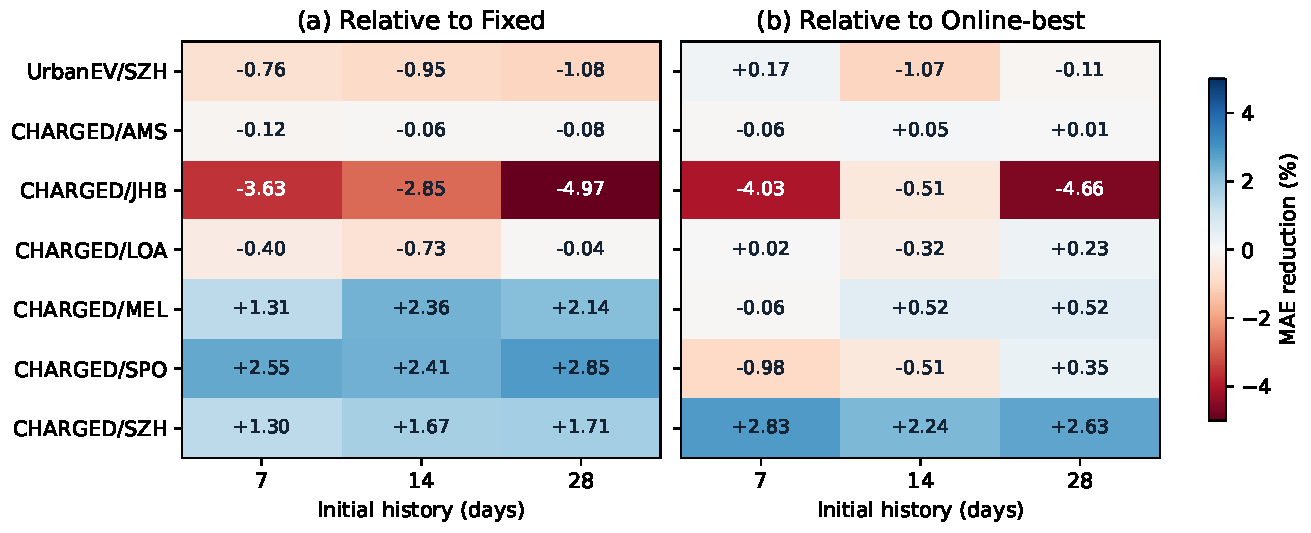
\includegraphics[width=\linewidth]{Images/selector-gains.pdf}
\caption{Historical retention switching versus Fixed and Online-best.}\label{fig:res-selector}\end{figure}

The \href{https://github.com/HungLD9505/adaptive-retention-ev/blob/52a91d3/report/full-results.csv}{historical results by group} give both contrasts for each history. The twelve-target Development study used a different control. Its fixed trajectory was selected on calibration targets and then compared with two selectors drawing on the same bank of independent trajectories. The past-MAE rule selected using past errors, while the confidence rule required evidence for switching.

\begin{table}[H]\centering\small
\caption{Selection from a common bank on twelve targets (MAE in kWh).}\label{tab:res-bank}
\begin{tabular}{lrrr}\toprule
History & Calibrated Fixed & Past MAE & Confidence rule\\\midrule
7 days & \textbf{3.3186} & 3.3234 & 3.3234\\
14 days & \textbf{3.2670} & 3.2904 & 3.2755\\
28 days & 3.3482 & 3.3252 & \textbf{3.3140}\\
\bottomrule\end{tabular}
\end{table}

The confidence rule improved on calibrated Fixed only at 28 days, where calibration had selected zero retention (Table~\ref{tab:res-bank}). At seven days the two selectors agree to four decimal places.

On the four previously inspected calibration targets, a separate experiment allocated the first 28 scheduled days to calibration, two to an embargo and the final 60 to evaluation. The embargo days remained part of causal replay. The four targets contributed 60, 22, 22 and 22 scored days in that final window, with equal weight per target after averaging seeds. Discrete selection reached 4.7983 kWh, calibrated Fixed 4.8031 and continuous selection 4.8062. Continuous exceeded Fixed by 0.00317 kWh. The discrete method used three branches and a different initialization and tuning budget, so this comparison cannot isolate the effect of coefficient continuity.

A separate \href{https://github.com/HungLD9505/adaptive-retention-ev/blob/52a91d3/docs/reports/issue99-decision-probe-20261110/handoff.md}{one-step decision experiment} cloned the current state before an update and compared following the continuous controller with holding its coefficient. Following reduced the next forecast error in 153 of 294 paired forecasts. The equal-target mean difference (follow minus hold) was $-0.000182$ kWh on these previously inspected calibration targets. In the persistent-shadow calibration, one of 57 completed decisions accepted a proposed change, from 69 proposals overall. Its mean MAE reduction against Fixed was 0.000118 kWh. Neither diagnostic establishes a practically useful decision threshold.


Figure~\ref{fig:issued-lambda} shows the coefficient recorded at each issued forecast for all four targets and all three seeds. Each point denotes an issued forecast; gaps indicate days without one. The dashed horizontal line marks the calibrated Fixed coefficient. These trajectories show how much the controller moved; the later-window MAEs above measure the forecasting consequence.
\begin{figure}[htbp]\centering
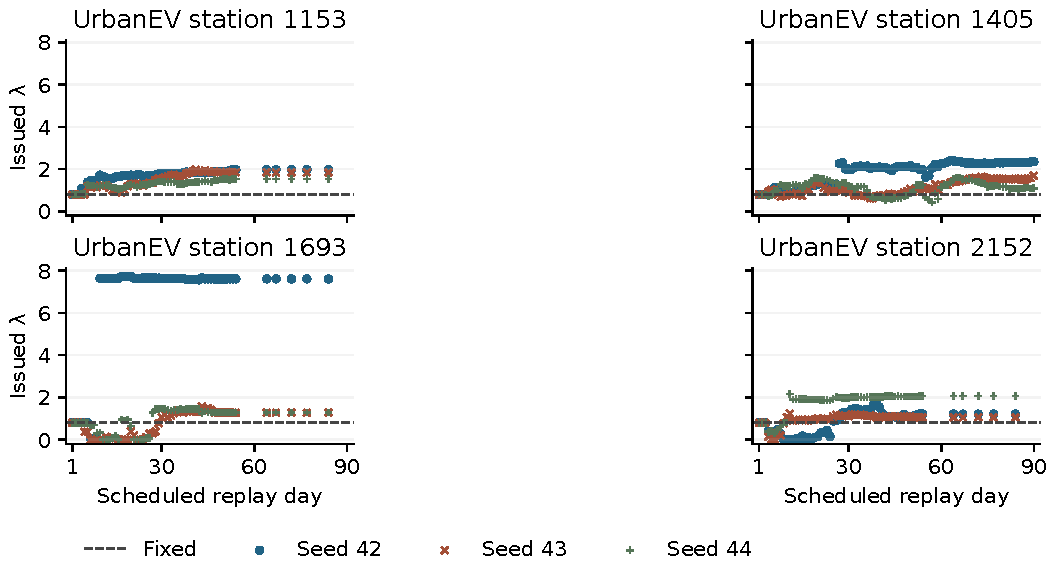
\includegraphics[width=.97\linewidth]{Images/issued-lambda.pdf}
\caption{Continuous retention coefficients at issued forecasts.}\label{fig:issued-lambda}
\end{figure}

\section{Combining two forecasts and adapting their weights}
The stable and fast GRUs differ in retention strength and in the history used for online updates. Static and adaptive fusion combine the same two forecast streams. Comparing either with single Fixed measures the overall change from using two experts. Comparing adaptive with static isolates the effect of updating their weights.

\begin{figure}[H]\centering
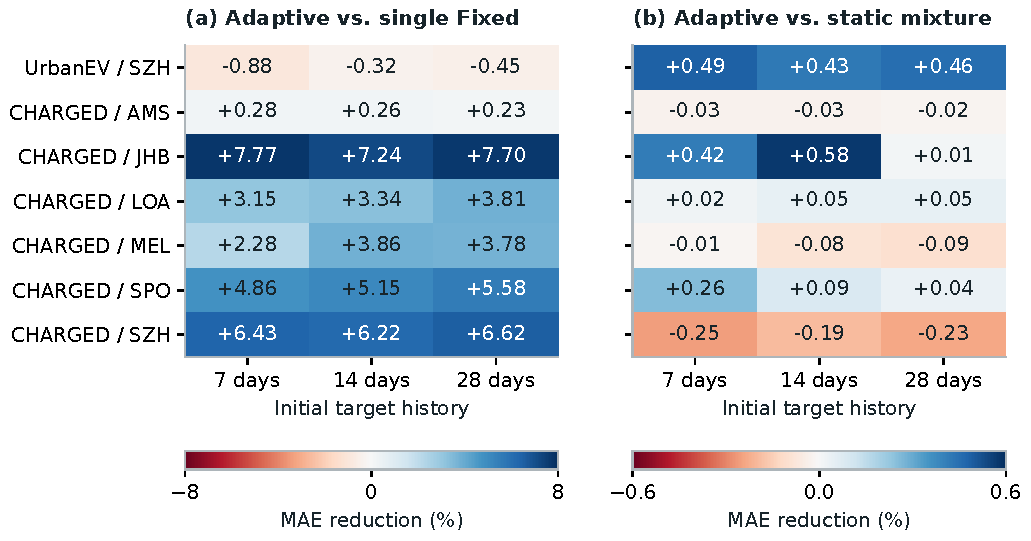
\includegraphics[width=.95\linewidth]{Images/cohort-comparisons.pdf}
\caption{Historical fusion gains. Color limits are $\pm8\%$ against Fixed and $\pm0.6\%$ against static fusion.}\label{fig:res-fusion}\end{figure}

Both mixtures improved on single Fixed in 18 of 21 historical groups. Adaptive fusion reduced MAE in all eighteen CHARGED groups (0.23--7.77\%) and increased it in all three UrbanEV groups (0.32--0.88\%). In the matched comparison, adaptive weights improved on static weights in twelve groups and increased error in nine. The panels in Figure~\ref{fig:res-fusion} use separate scales because the weighting differences are smaller.

At 14 days in UrbanEV/SZH, adaptive weighting improved the static mean from 8.0361 to 8.0016 kWh, yet single Fixed reached 7.9758. In CHARGED/MEL, adaptive fusion reached 52.2649 kWh compared with 54.3655 for single Fixed and 52.2222 for static fusion. The two examples show why a win count depends on the control. Posthoc resampling across entities gave intervals spanning zero in thirteen of the 21 adaptive-versus-static comparisons.

\clearpage
\subsection{Examples across forecast dates}

\begin{figure}[H]\centering
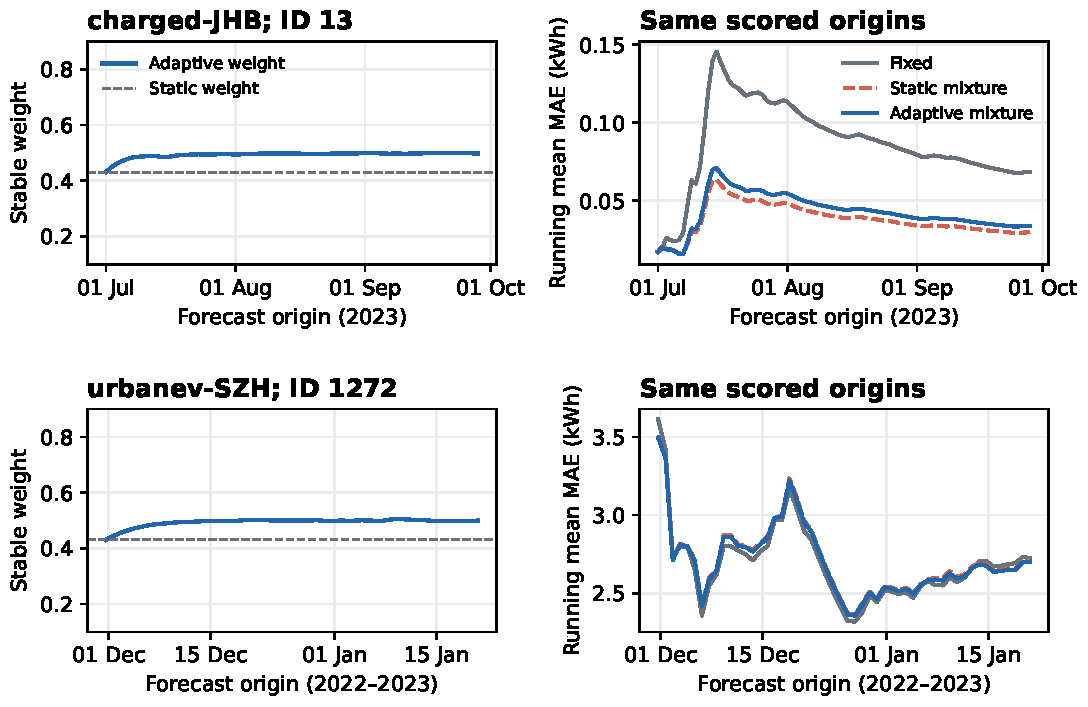
\includegraphics[width=.95\linewidth]{Images/trajectories.pdf}
\caption{Historical expert weights and running mean daily errors at two targets.}\label{fig:res-traces}\end{figure}

Figure~\ref{fig:res-traces} follows JHB identifier 13 and UrbanEV identifier 1272 at 14 days with seed 42. Within each group, the selection rule used the upper median of the entity-level gains against Fixed among targets with Fixed MAE above $10^{-4}$ kWh. The displayed seed illustrates the trajectory. Target selection used gains averaged across seeds. Weights at each forecast origin use only feedback available by that time. The running mean divides the sum of daily MAEs by the number of scored origins to date. Each trace illustrates one target, while the group comparisons average over targets and seeds.

A bounded follow-up on the twelve Development targets at 14 days compared alternative weight updates. AdaHedge \cite{rooij2014} reduced MAE from 3.291048 to 3.284880 kWh relative to the original adaptive rule. Single Fixed achieved 3.267000 kWh, so the alternative did not meet its criterion for further evaluation.

\clearpage
\section{Evaluation on additional Development targets}
The follow-up fixed both controls, the forecast recipe and the 46 target identifiers before evaluating their outcomes. At the 14-day budget, 3,948 of 4,140 scheduled identifier--day pairs had complete outcomes. These targets came from the same seven dataset--city groups and evaluation calendar, so the follow-up tests performance on additional identifiers within that setting. Table~\ref{tab:res-confirm} shows group MAE in kWh and percentage reductions relative to each control. Bold marks the lowest MAE in each row.

\begin{table}[H]\centering\small
\caption{Forecast errors on the 46 additional Development identifiers.}\label{tab:res-confirm}
\resizebox{\linewidth}{!}{\begin{tabular}{@{}lrrrrrrr@{}}\toprule
Group & IDs & Fixed & Fast & Static & Adaptive & vs Fixed (\%) & vs static (\%)\\\midrule
UrbanEV/SZH & 10 & \textbf{7.4023} & 8.8496 & 8.1106 & 7.9944 & -8.00 & +1.43\\
CHARGED/AMS & 10 & 16.2823 & \textbf{16.2107} & 16.2287 & 16.2344 & +0.29 & -0.03\\
CHARGED/JHB & 1 & 8.0410 & 8.4356 & 7.9544 & \textbf{7.9147} & +1.57 & +0.50\\
CHARGED/LOA & 10 & 2.0621 & 2.1082 & 2.0371 & \textbf{2.0317} & +1.48 & +0.26\\
CHARGED/MEL & 4 & \textbf{10.9073} & 11.6425 & 11.1002 & 11.0267 & -1.10 & +0.66\\
CHARGED/SPO & 1 & 8.4985 & \textbf{7.6644} & 7.7956 & 7.8368 & +7.79 & -0.53\\
CHARGED/SZH & 10 & 4.2698 & 4.3512 & 4.1675 & \textbf{4.1578} & +2.62 & +0.23\\
\bottomrule\end{tabular}}
\end{table}

Adaptive fusion improved on single Fixed in five of seven groups and on static fusion in five of seven. The groups differed between comparisons. In UrbanEV/SZH, it reduced error by 1.43\% against static fusion but increased it by 8.00\% against Fixed. In SPO, it reduced error by 7.79\% against Fixed and increased it by 0.53\% against static. SPO and JHB each contributed one identifier, so each of those group means describes a single target.

Figure~\ref{fig:locked-intervals} shows both primary intervals on the same scale. Positive values favour adaptive fusion.
\begin{figure}[htbp]\centering
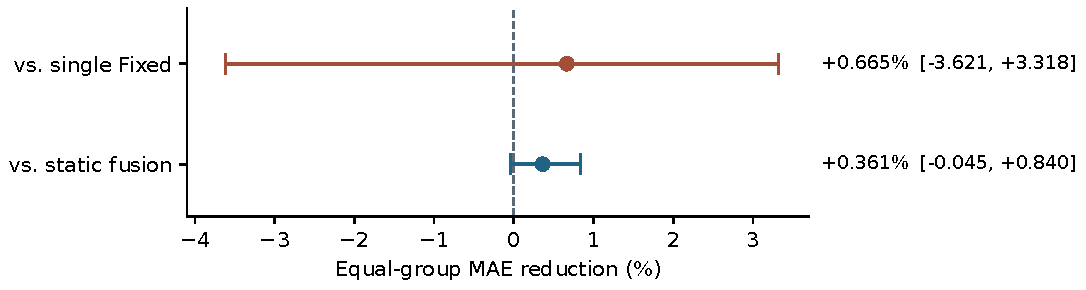
\includegraphics[width=.97\linewidth]{Images/locked-intervals.pdf}
\caption{Adaptive fusion on 46 targets: estimates and nominal 97.5\% intervals.}\label{fig:locked-intervals}
\end{figure}

Giving each dataset--city group equal weight, adaptive fusion reduced MAE by 0.6653\% relative to single Fixed and 0.3610\% relative to static. 

The paired resampling analysis gave nominal 97.5\% intervals of $[-3.6209,3.3176]\%$ and $[-0.0449,0.8399]\%$, respectively. The prespecified criterion required both lower bounds to exceed zero. The prespecified three-day sensitivity intervals also included zero. At fourteen days each comparison had two undefined replicates out of 10,000, leaving both sensitivity intervals undefined. Both primary intervals include zero, so the evaluation did not establish superiority to both controls. The more consistent empirical finding across the chapter is the benefit of source initialization under short target histories. The added benefit of adapting retention or forecast weights depends on the target group and the comparator.

\chapter{Conclusion}\label{chap:conclusion}

\section{Summary of Achievements}

A charging station with one week of records offers few examples from which to learn its daily demand pattern. This thesis examined how much a forecaster can learn from established locations and whether recent forecast errors can tell it when to relax the influence of that prior training.

Source initialization gave the clearest improvement. On twelve UrbanEV targets, a GRU initialized from other locations reduced mean absolute error by 33.35\%, 31.64\% and 29.80\% with 7, 14 and 28 days of target history, respectively. Source initialization improved the seed-averaged error at all twelve targets for the seven- and fourteen-day budgets and at eleven targets for the twenty-eight-day budget. Both the transferred GRU and the target-only GRU had their initial training budgets selected on separate calibration targets. Even with 28 days of local observations, the transferred model retained an advantage for next-day hourly forecasts.

Once target training begins, the retention coefficient $\lambda$ controls how strongly the target encoder is penalized for departing from the source representation. On four calibration targets, $\lambda \approx 0.798$ gave the lowest error among 21 tested values. In the historical evaluation, switching coefficients on the basis of recent errors and their uncertainty improved on a constant $\lambda=1$ in nine of 21 dataset--city and history combinations. The rule improved on Online-best in eleven of the same 21 combinations. On twelve additional UrbanEV targets, a confidence rule selecting among the same candidate trajectories as the calibrated fixed control achieved lower error at 28 days and higher error at 7 and 14 days. These comparisons identify settings in which switching helped. They leave open how to recognize those settings before the next forecast.

A second approach combined forecasts from two GRUs with the same learning rate but different retention coefficients and online training windows. Both static and adaptive weighting improved on a single fixed-retention GRU in 18 of the 21 historical groups. With the same two expert forecasts, adaptive fusion improved on the calibrated static blend in twelve groups. On twelve UrbanEV Development targets at fourteen days, equal weighting reproduced the adaptive MAE within 0.000007 kWh. Historical comparisons with equal weighting favored the adaptive rule in all 21 groups, with reductions of at most 0.263\%. A follow-up evaluation fixed the methods and selected 46 additional Development identifiers before examining their outcomes. At 14 days of history, adaptive weighting reduced error by 0.67\% against the single fixed model and 0.36\% against the static mixture, giving each dataset--city group equal weight. Both 97.5\% uncertainty intervals included zero. The follow-up therefore leaves the incremental benefit of adapting the weights uncertain.

\section{Limitations and Future Work}

We simulated cold start by restricting how much recorded history the forecaster could use. A station's first day in an evaluation window may fall well after it opened. CHARGED also includes values interpolated or filled by the data publisher \cite{charged2025}. Our replay enforces label availability on the released series; the real-time availability of each upstream estimate cannot be reconstructed from that series. Following stations with verified opening dates would test whether source initialization also helps during the first weeks of operation, when customers are still discovering the site.

The historical groups were revisited during method development. The 46 additional identifiers provided a separate evaluation at the same seven dataset--city groups and during the same calendar period. Johannesburg and S\~ao Paulo each contributed a single identifier to that follow-up, which limits what their results can tell us about variation within either city. Evaluating a prespecified rule in a later period or in an additional city would test how well the observed effects carry over.

The one-step follow-versus-hold diagnostic found a mean advantage of only 0.000182 kWh on the calibration targets. A prospective test on additional targets or a later period would record each proposed change in $\lambda$ before the next block of forecasts. Starting from the same model state, one copy would adopt the proposed coefficient and another would keep the current value. Scoring both on the same subsequent days would show whether the evidence available at decision time predicts a benefit from switching. That prospective comparison would address the question left open here: when can a station with little history safely rely less on its source model?

% ---------- References ----------
\appendix
\chapter{Continuous retention diagnostic}\label{app:continuous}
The four-target diagnostic changes a real-valued coefficient on one target branch. From current real parameters and Adam moments it creates a virtual update using two older complete arrived days $A$. A newer complete arrived day $V$, not yet used in real training, supplies the forecast validation loss. Following the one-step hypergradient approach \cite{luketina2016}, the diagnostic computes
\begin{equation}\begin{aligned}
\widetilde\theta_t(\lambda)&=\operatorname{AdamStep}
\left(\theta_t,m_t,v_t;\nabla_\theta[F_A+\lambda R_A]\right),\\
g_t&=\left.\frac{\partial F_V(\widetilde\theta_t(\lambda))}
{\partial\lambda}\right|_{\lambda_t},\\
\lambda_{t+1}&=\Pi_{[0,U]}\left(\lambda_t-\eta_\lambda g_t\right).
\end{aligned}\label{eq:hypergradient}\end{equation}
Previous parameters and moments are fixed starting state for this local derivative. The differentiable virtual Adam step uses bias-corrected moments and does not mutate the real optimizer. After the decision, real training consumes the newly arrived example; the next forecast uses only permitted data.

The fixed search defines $U=33.84425$ and supplies its minimizer as $\lambda_0=0.798445$. Calibration compares three nominal step fractions at two decision cadences and selects $\eta_\lambda=211.295$ with an update at each eligible arrival. Across 801 forecast records for the continuous branch, the deployed coefficients ranged from 0 to 7.73128. The coefficient step size differs from the model learning rate 0.001. Adam uses betas $(0.9,0.999)$ and optimizer epsilon $10^{-8}$, separate from retention epsilon 0.001. The controller upper bound is the smallest measured coefficient above the selected Fixed value that is harmful relative to zero; if none is measured, it uses the largest finite tested coefficient. Here the fallback gives the stated upper endpoint. Step sizes are scaled from a calibration-prefix hypergradient pilot and selected across three nominal step fractions and two cadences. The projection interval is a study-specific bounded domain, not a paper-established EV constant or a measured claim that every value in it is useful.



\chapter{Experimental evidence index}\label{app:evidence}
The linked records give the run-level errors or aggregates used in Chapter~\ref{chap:results}. Each link points to the same repository revision so the reported results can be traced to a fixed snapshot.

\begin{table}[H]\centering\small
\caption{Result tables, figures and supporting records.}
\begin{tabularx}{\linewidth}{@{}l l X@{}}\toprule
Comparison & Location & Evidence\\\midrule
Backbone MAE & Table~\ref{tab:baselines} & \href{https://github.com/HungLD9505/adaptive-retention-ev/tree/0167b5189ed519490ba8361a70e0656c6d7e5850/docs/reports/issue99-teacher-review-20261111}{Independent benchmark summaries}\\
Source initialization & Table~\ref{tab:res-transfer} & \href{https://github.com/HungLD9505/adaptive-retention-ev/blob/0167b5189ed519490ba8361a70e0656c6d7e5850/docs/reports/issue99-history-review-20261110/cells.csv}{MAE by history, target, seed and method}\\
Retention calibration & Figure~\ref{fig:res-fixed} & \href{https://github.com/HungLD9505/adaptive-retention-ev/blob/0167b5189ed519490ba8361a70e0656c6d7e5850/docs/reports/issue99-study-20261110/fixed-trials.csv}{Measured coefficients and gradient ratios}\\
Retention switching & Figure~\ref{fig:res-selector} & \href{https://github.com/HungLD9505/adaptive-retention-ev/blob/0167b5189ed519490ba8361a70e0656c6d7e5850/report/full-results.csv}{Historical group scores and intervals}\\
Historical fusion & Figure~\ref{fig:res-fusion} & \href{https://github.com/HungLD9505/adaptive-retention-ev/blob/0167b5189ed519490ba8361a70e0656c6d7e5850/docs/reports/issue99-full-scope-20261110/group-results.csv}{Group MAEs and paired reductions}\\
Historical controls & Section~\ref{sec:weight-controls} & \href{https://github.com/HungLD9505/adaptive-retention-ev/blob/0167b5189ed519490ba8361a70e0656c6d7e5850/docs/reports/issue99-teacher-review-20261111/fusion-controls-groups.csv}{Equal weighting and sharing alone}\\
Development controls & Table~\ref{tab:weight-controls} & \href{https://github.com/HungLD9505/adaptive-retention-ev/blob/0167b5189ed519490ba8361a70e0656c6d7e5850/docs/reports/issue123-bounded-weighting-20261113/development-mae.csv}{Target- and seed-level weighting results}\\
Locked evaluation & Table~\ref{tab:res-confirm} & \href{https://github.com/HungLD9505/adaptive-retention-ev/tree/0167b5189ed519490ba8361a70e0656c6d7e5850/docs/reports/issue119-confirmation-20261113}{Group and identifier results, intervals and verification}\\
\bottomrule\end{tabularx}\end{table}


\bibliographystyle{IEEEtran}
\renewcommand{\bibname}{References}
\clearpage
\phantomsection
\addcontentsline{toc}{chapter}{References}
\bibliography{references}

\end{document}
